\section{Data Warehouse Implementation}

\begin{frame}{Efficient Data-Cube Computation}
	\begin{itemize}
		\item \textbf{Data cube can be viewed as a lattice of cuboids.}
		\item The bottom-most cuboid is the base cuboid.
		\item The top-most cuboid (apex) contains only one cell.
		\item How many cuboids in an $n$-dimensional cube with $L_i$ levels associated with dimension $i$?
		      \begin{align}
			      T = \prod_{i=1}^{n} (L_i +1).
		      \end{align}
		\item \textbf{{\color{airforceblue}Materialization} of data cube.}
		      \begin{itemize}
			      \item Materialize each (cuboid) (full materialization), \\
			            none (no materialization), or some (partial materialization).
			      \item Selection of cuboids to materialize based on size, sharing, access frequency, etc.
		      \end{itemize}
	\end{itemize}
\end{frame}

\begin{frame}{The "Compute Cube" Operator}
	\begin{columns}
		\begin{column}{0.6\textwidth}
			\vspace{-4.8cm}
			\begin{itemize}
				\item \textbf{Cube definition and computation in DMQL:} \\
				      \texttt{DEFINE CUBE sales [item, city, year]:}\\
				      \texttt{SUM (sales$\_$in$\_$dollars);}\\
				      \texttt{COMPUTE CUBE sales;}
				\item \textbf{Transform it into an SQL-like language:}\\
				      with a new operator \texttt{CUBE BY} (Gray et al. 96).\\
				      \texttt{SELECT item, city, year, SUM (amount)}\\
				      \texttt{FROM sales}\\
				      \texttt{CUBE BY item, city, year;}
				\item \textbf{Need to compute the following} \texttt{GROUP BY}\textbf{s:}\\
				      \texttt{(city, item, year),}\\
				      \texttt{(city, item), (city, year),}\\
				      \texttt{(item, year),}\\
				      \texttt{(city), (item), (year)}\\
				      \texttt{()}
			\end{itemize}
		\end{column}
		\begin{column}{0.3\textwidth}  %%<--- here
			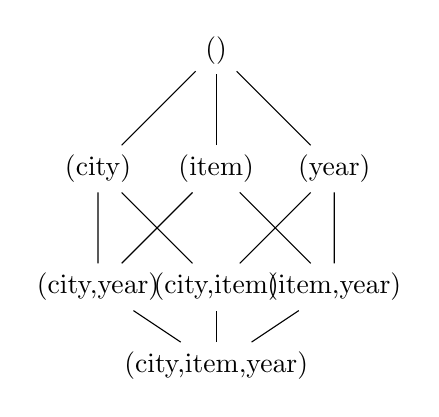
\begin{tikzpicture}
				\node at (0,0) (a) {()};
				\node at (0,-1.5) (b) {(item)};
				\node at (-1.5,-1.5) (c) {(city)};
				\node at (1.5,-1.5) (d) {(year)};
				\node at (0,-3) (e) {(city,item)};
				\node at (-1.5,-3) (f) {(city,year)};
				\node at (1.5,-3) (g) {(item,year)};
				\node at (0,-4) (h) {(city,item,year)};
				\draw (a) -- (c) -- (f) -- (h);
				\draw (h) -- (g) -- (d) -- (a);
				\draw (h) -- (e);
				\draw (e) -- (c);
				\draw (e) -- (d);
				\draw (f) -- (b);
				\draw (g) -- (b);
				\draw (b) -- (a);
			\end{tikzpicture}
		\end{column}
	\end{columns}
\end{frame}

\begin{frame}{Indexing OLAP Data: Bitmap Index}
	\begin{itemize}
		\item \textbf{Index on a particular column.}
		\item \textbf{Each value in the column has a bit vector: bit-op is fast.}
		\item \textbf{Length of bit vector: $\#$ of records in base table.}
		\item \textbf{$i$-th bit set, if $i$-th row of base table has value of bit vector.}
		\item \textbf{Not suitable for high-cardinality domains:}
		      \begin{itemize}
			      \item A bit compression technique called Word-Aligned Hybrid (WAH) makes it work for high-cardinality domain as well [Wu et al., TODS'06].
		      \end{itemize}
	\end{itemize}
	\centering
	\textbf{Base table} \hspace{2.5cm} \textbf{Index on region} \hspace{2.5cm} \textbf{Index on type}\\
	\begin{tabular}{| c | c | c |}
		\hline
		\textbf{Cust} & \textbf{Region} & \textbf{Type} \\\hline
		$C1$          & Asia            & Retail        \\\hline
		$C2$          & Europe          & Dealer        \\\hline
		$C3$          & Asia            & Dealer        \\\hline
		$C4$          & America         & Retail        \\\hline
		$C5$          & Europe          & Dealer        \\\hline
	\end{tabular}\hspace{0.1cm}
	\begin{tabular}{| c | c | c | c |}
		\hline
		\textbf{RecID} & \textbf{Asia} & \textbf{Europe} & \textbf{America} \\\hline
		1              & 1             & 0               & 0                \\\hline
		2              & 0             & 1               & 0                \\\hline
		3              & 1             & 0               & 0                \\\hline
		4              & 0             & 0               & 1                \\\hline
		5              & 0             & 1               & 0                \\\hline
	\end{tabular}\hspace{0.1cm}
	\begin{tabular}{| c | c | c |}
		\hline
		\textbf{RecID} & \textbf{Retail} & \textbf{Dealer} \\\hline
		$1$            & 1               & 0               \\\hline
		$2$            & 0               & 1               \\\hline
		$3$            & 0               & 1               \\\hline
		$4$            & 1               & 0               \\\hline
		$5$            & 0               & 1               \\\hline
	\end{tabular}
\end{frame}

\begin{frame}{Indexing OLAP Data: Join Indices}
	\begin{itemize}
		\item \textbf{Join index:}
		      \begin{align}
			      \text{JI}(\texttt{R-id}, \texttt{S-id}) \quad \text{where} \quad \text{R}(\texttt{R-id}, \ldots) \bowtie  \text{S}(\texttt{S-id}, \ldots).
		      \end{align}
		\item \textbf{Traditional indices map the values to a list of record ids.}
		      \begin{itemize}
			      \item Materializes relational join in JI-file and speeds it up.
		      \end{itemize}
		\item \textbf{In data warehouses, join index relates the values of the dimensions \\ of a star schema to rows in the fact table.}
		      \begin{itemize}
			      \item E.g. fact table: Sales and two dimensions location and item.
			            \begin{itemize}
				            \item A join index on location maintains for each distinct location a list of \texttt{R-ids} of the tuples recording the sales in that location.
			            \end{itemize}
			      \item Join indices can span multiple dimensions.
		      \end{itemize}
	\end{itemize}
\end{frame}

\begin{frame}{Indexing OLAP data: Join Indices (Example)}
	\centering
	\begin{tikzpicture}
		\node[basic, rectangle split part fill={red!20,white}] at (2,2) (sales) {sales
			\nodepart{second}
			~\\
			~\\
			~\\
			T57\\
			~\\
			~\\
			T238
			~\\
			~\\
			T249
			~\\
			~\\
			~\\
			T884\\
			~};

		\node[basic, rectangle split part fill={green!20,white}] at (-2,1) (location) {location
			\nodepart{second}
			~\\
			~\\
			~\\
			Main street\\
			~\\
			~\\
			~};

		\node[basic, rectangle split part fill={yellow!20,white}] at (6,1) (item) {item
			\nodepart{second}
			~\\
			~\\
			~\\
			Sony-TV\\
			~\\
			~\\
			~};

		\draw (-1,0.8) -- (1,1);
		\draw (-1,0.8) -- (1,1.9);
		\draw (-1,0.8) -- (1,2.9);

		\draw (5,1) -- (1.5,2.9);
		\draw (5,1) -- (1.8,1.9);
	\end{tikzpicture}
\end{frame}

\begin{frame}{Efficient Processing of OLAP Queries}
	\begin{itemize}
		\item \textbf{Determine which operations should be performed on the available cuboids.}
		      \begin{itemize}
			      \item Transform drill, roll, etc. into corresponding SQL and/or OLAP operations.\\
			            E.g. \texttt{dice} $=$ \texttt{selection} $+$ \texttt{projection}.
		      \end{itemize}
		\item \textbf{Determine which materialized cuboid(s) should be selected for OLAP operation.}
		      \begin{itemize}
			      \item Let the query to be processed be on \texttt{\{brand, province\_or\_state\}} with the condition \texttt{"year = 2004"}, and there are $4$ materialized cuboids available:
			            \begin{itemize}
				            \item[1)] \texttt{{year, item\_name, city}}.
				            \item[2)] \texttt{{year, brand, country}}.
				            \item[3)] \texttt{{year, brand, province\_or\_state}}.
				            \item[4)] \texttt{{item\_name, province\_or\_state} where year $=$ 2004}.
			            \end{itemize}
			      \item Which should be selected to process the query?
		      \end{itemize}
		\item \textbf{Explore indexing structures and compressed vs. dense-array structures in MOLAP.}
	\end{itemize}
\end{frame}

\begin{frame}{OLAP Server Architectures}
	\begin{itemize}
		\item \textbf{Relational OLAP (ROLAP).}
		      \begin{itemize}
			      \item Use relational or extended-relational DBMS to store \\
			            and manage warehouse data and OLAP middleware.
			      \item Include optimization of DBMS backend, implementation of aggregation navigation logic, and additional tools and services.
			      \item Greater scalability.
		      \end{itemize}
		\item \textbf{Multidimensional OLAP (MOLAP).}
		      \begin{itemize}
			      \item Sparse array-based multidimensional storage engine.
			      \item Fast indexing to pre-computed summarized data.
		      \end{itemize}
		\item \textbf{Hybrid OLAP (HOLAP) (e.g., Microsoft SQL-Server).}
		      \begin{itemize}
			      \item Flexibility, e.g., low level: relational, high-level: array.
		      \end{itemize}
		\item \textbf{Specialized SQL servers (e.g., Redbricks).}
		      \begin{itemize}
			      \item Specialized support for SQL queries over star/snowflake schemas.
		      \end{itemize}
	\end{itemize}
\end{frame}
